\documentclass[a4paper,oneside,article,11pt]{memoir}
\usepackage[english]{babel}
\usepackage[utf8]{inputenc}
\usepackage{amsmath,amssymb,amsthm}

% This font looks so good.
\usepackage[sc]{mathpazo}

% Typesetting pseudo-code
\usepackage{algorithm}
\usepackage{algorithmic}
\usepackage{multirow}
% Code comments like [CLRS]
\renewcommand{\algorithmiccomment}[1]{\makebox[5cm][l]{$\triangleright$ \textit{#1}}}
\usepackage{framed,graphicx,xcolor}
\usepackage[font={small,it}]{caption}
\usepackage{listings}
\usepackage{units}

% Relative references
\usepackage{varioref}

\usepackage{hyperref}

\bibliographystyle{plain}

\title{Advanced Data Structures \\ Project 1 - Fibonacci heaps}
\author{Peter Gabrielsen 20114179 \\
Christoffer Hansen 20114637}
\newcounter{qcounter}
\begin{document}

\begin{titlingpage}
\clearpage

\maketitle
\thispagestyle{empty}

\begin{abstract}
ABSTRACT HERE
\\
\\
\\
The code can be found at: \\\url{CODE HERE}.
\end{abstract}
\end{titlingpage}

\pagebreak

\tableofcontents

\pagebreak

\chapter{Introduction}
INTRO

\chapter{Implementation}
We will in this section describe and discuss the design choices of our implementations of the binary heap and the Fibonacci heap.
\subsection{Binary heap}
The binary heap by Williams~\cite{williams} was implemented as a minimum heap using the pseudo code in CLRS~\cite[p.~151-170]{clrs}. Using this implementation we get the following time bounds for the heap operations:

\begin{figure}[H]
\centering
\begin{tabular}{l|c}
Operation & Bound \\\hline
\texttt{Insert} & $\mathcal{O}(\log n)$ \\\hline
\texttt{FindMin} & $\mathcal{O}(1)$ \\\hline
\texttt{DeleteMin} & $\mathcal{O}(\log n)$ \\\hline
\texttt{DecreaseKey} & $\mathcal{O}(\log n)$
\end{tabular}
\caption{Time bounds of the binary heap.}
\end{figure}

In order to implement the decrease key operation we need some way to find the node in the binary heap corresponding to a node in our graph. To do this we have a table which given a node id from our graph gives us the index in the binary heap of that node id. We can then call decrease key. This way of implementing it gives an overhead in space usage of $n$, where $n$ is the number of vertices in the graph.

\subsection{Fibonacci heap}

\chapter{Experimental setup}
\label{chtp:experiment_setup}
%TODO write something about the machine which ran the experiments and something about how we measure the different things. Maybe copy all this from the AE report?

The experiments were performed on a machine with a Intel i5-3210M @ 2.5GHz (Ivy Bridge) with 128K bytes of L1 cache, 512K bytes of L2 and 3072K bytes of L3 cache. The machine had 4.2GB ram and ran Ubuntu 14.04 with kernel version 3.16.0-50.

The running time was measured using the built in \texttt{high\_resolution\_clock} in the \texttt{chrono} library. This measures the wall clock. It is the clock in \texttt{c++} with the highest precision, i.e. the shortest tick period.

The code is compiled with \texttt{g++ 4.8.4} with the \texttt{c++11} standard enabled and no optimization level.

The elements in our data structures were 32 bit integers. Random elements were generated uniformly in the 32 bit integer range using the Mersenne Twister 19937 from the \texttt{random} library.

CPU measurements were collected using \texttt{PAPI 5.3.0.0}

We used \texttt{perf} to measure page faults.


\chapter{Worst case time bounds of the heaps}
In this section we will argue about how the algorithms perform in the worst case as opposed to the amortized time bounds. We will for each operations on the heaps argue how the worst cases are obtained.

\subsection{\texttt{FindMin}}
Finding the minimum element is in both the Fibonacci heap and the binary heap a constant time operation. We keep a pointer to the minimum element in the Fibonacci heap and in the binary heap we just return the first element in the array which holds the heap.

\subsection{\texttt{Insert}}
Inserting into the binary heap is simple. We insert the element at the last position in the binary tree, i.e. the heap, and bubble the element up to its correct position. In the worst case we need to bubble the element to the top, which means bubbling through $\mathcal{O}(\log n)$ layers which gives a logarithmic complexity in the worst case for this operation.

Inserting in the Fibonacci heap is even simpler. We simply just add the element to the root list which just involves manipulating a doubly linked list, i.e. some pointer calculations. 
%This constant time operation is what allows us to give the amortized analysis of decrease key?

\subsection{\texttt{DeleteMin}}
Delete the minimum element is $\mathcal{O}(\log{n})$ for the binary heap and $\mathcal{O}(\log{n})$ amortized for the Fibonacci heap. This upper bound is trivially obtained in the binary heap by having the heap ordered as a sorted array. This way, whenever we delete the minimum we would move the largest element to the top and bubble it $\log n$ levels down again to the bottom.

It can however be extremely expensive to delete the minimum in the Fibonacci heap. When we delete the minimum from a Fibonacci heap we need to consolidate the heap. This operations is linear in the size of the root list. The root list can grow linearly in the worst case if we do $n$ inserts in a row, then the root list will contain at least $n$ nodes, which needs to be consolidated in time $\mathcal{O}(\vert root\_list \vert)$.

\subsection{\texttt{DecreaseKey}}
Decreasing a key in the binary heap is done by giving the element a new priority and then bubble it up to its new position. The worst case is that the element decreased is the last element and its new priority is the lowest in the tree, which means that it needs to bubble to the top of the heap. This costs $\mathcal{O}(\log n)$.

The worst case for the Fibonacci heap would be if we have a tree of height $\mathcal{O}(\log n)$ where every internal node on the path to the lowest leaf, which is decreased, is marked. This will cause a chain of cuts and cascading cuts all the way up to the root, which will take $\mathcal{O}(\log n)$ time.

\chapter{Heap experiments}
In this section we will design and perform experiments where we try to measure the running time and number of comparisons of the operations for both our priority queue implementations. We will give a summary of the design of each experiment, results, and discussion of the found results for each operation.

\subsection{\texttt{FindMin}}
Since finding the minimum element of both queues are constant time operations and basically just dereferencing a pointer we did not think it made sense to compare the running times in terms of wall clock. What we did instead is we measured the number of cycles for performing a single FindMin operation and the number of conditional branching operations needed. We would highly expect that the results do not depend on the size of the heap, why we made an experiment where the size of the heap were powers of two in the range from $\left[2^0, 2^{22}\right]$. The experiment were repeated 10000 times and averaged. The results can be found in figure~\ref{fig:findmin_cycles} and~\ref{fig:findmin_br}.
Our hypothesis were fortunately true and we do not think that there is much to discuss about the results.

\begin{figure}[H]
\centering
\begin{minipage}{0.48\columnwidth}
  \centering
  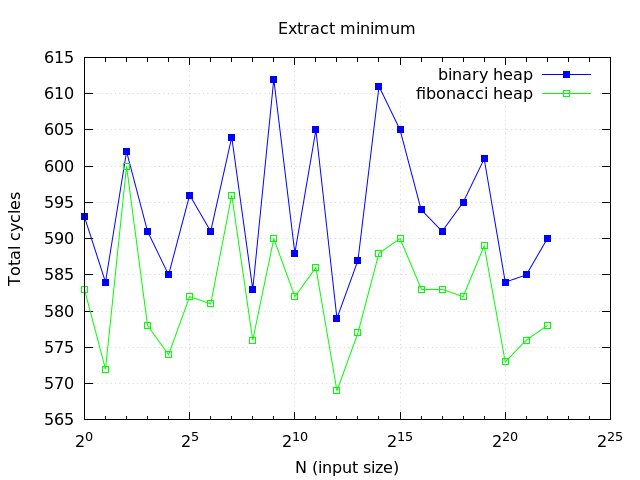
\includegraphics[width=\linewidth]{../res/findmin/extract_min_cycles.png}%
  \caption{The number of cycles fluctuates a little but this is to be expected.}
  \label{fig:findmin_cycles}
\end{minipage}%
\hfill
\begin{minipage}{0.48\columnwidth}
  \centering
  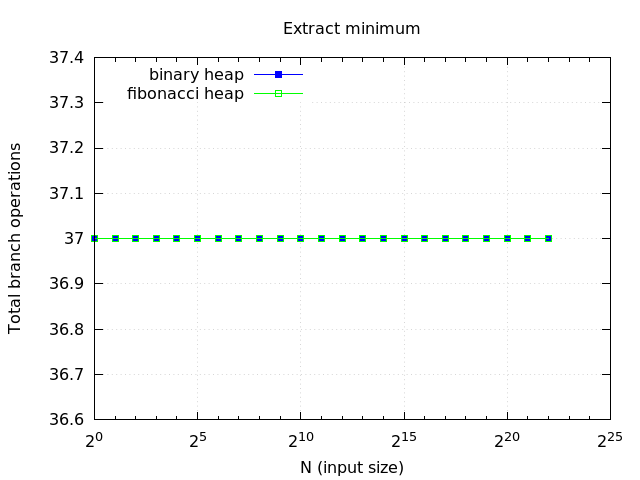
\includegraphics[width=\linewidth]{../res/findmin/extract_min_branch.png}%
  \caption{It took exactly 37 branch operations to measure extract the minimum element.}
  \label{fig:findmin_br}
\end{minipage}
\end{figure}

\subsection{\texttt{Insert}}
Inserting in the Fibonacci heap is a constant time operation while inserting into the binary heap is logarithmic. We would like to see that the binary heap performs worse. We will test both priority queues in both the average case and the worst case. In the average case we select a random priority in the integer range and insert it into the heap.
%TODO how high can we expect the elemen to bubble on average?
In the worst case we insert elements into the heap in reverse order. This will cause the elements to bubble all the way to the top on every insert.

The experiments are repeated 100 times and the results are averaged. We plot the y-axis to depict the amount of time a single insert takes or how many branch operations are performed per insert.

We expect to see that the Fibonacci heap is constant time in any case and that the binary heap is logarithmic in both cases. The number of comparisons performed in the Fibonacci heap should therefore also be constant on each insert while the number of comparisons in the binary heap should increase logarithmically in the size of the input and increase even more drastically in the worse case.

The results can be found in figure~\ref{fig:insert_t_random},~\ref{fig:insert_t_worst},~\ref{fig:insert_b_random}, and~\ref{fig:insert_b_worst}.

\begin{figure}[H]
\centering
\begin{minipage}{0.48\columnwidth}
  \centering
  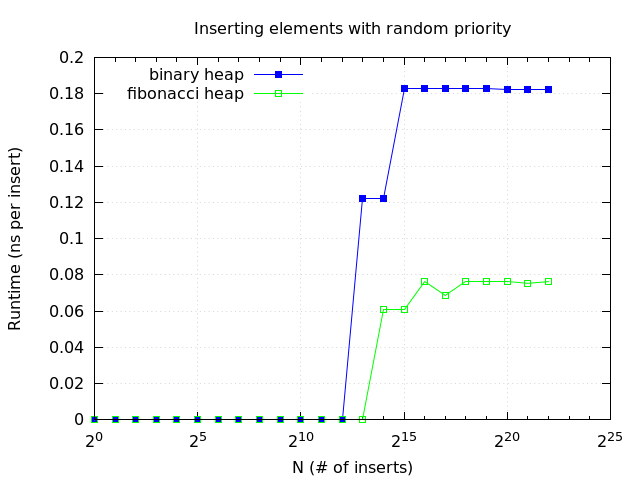
\includegraphics[width=\linewidth]{../res/inserts/insert_random_time.png}%
  \caption{Inserting $n$ elements with random priority and the number of nanoseconds per insert.}
  \label{fig:insert_t_random}
\end{minipage}%
\hfill
\begin{minipage}{0.48\columnwidth}
  \centering
  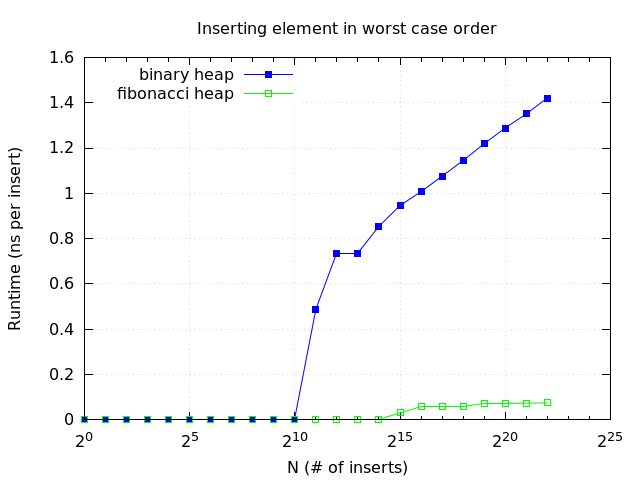
\includegraphics[width=\linewidth]{../res/inserts/insert_worst_time.png}%
  \caption{Inserting $n$ elements in reversed order and the number of nanoseconds per insert.}
  \label{fig:insert_t_worst}
\end{minipage}
\end{figure}

\begin{figure}[H]
\centering
\begin{minipage}{0.48\columnwidth}
  \centering
  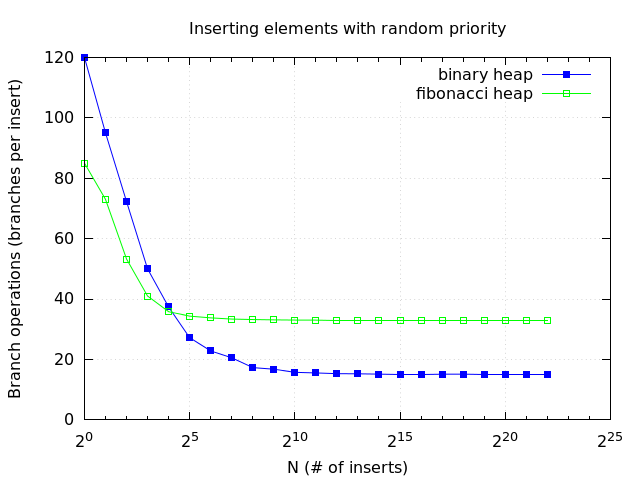
\includegraphics[width=\linewidth]{../res/inserts/insert_random_branch.png}%
  \caption{Inserting $n$ elements with random priority and the number of branch operations per insert.}
  \label{fig:insert_b_random}
\end{minipage}%
\hfill
\begin{minipage}{0.48\columnwidth}
  \centering
  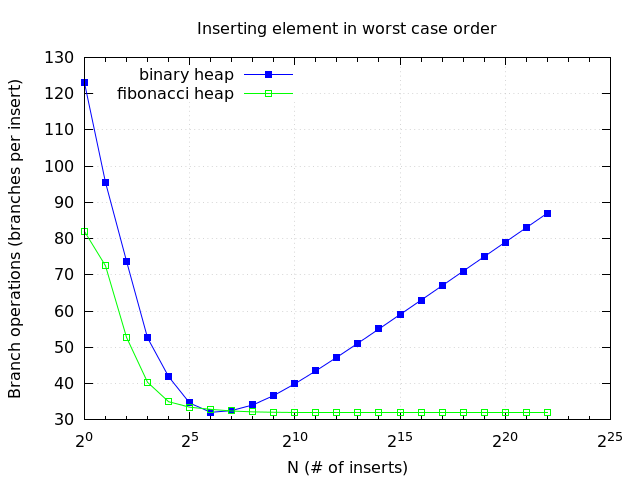
\includegraphics[width=\linewidth]{../res/inserts/insert_worst_branch.png}%
  \caption{Inserting $n$ elements in the reversed order and the number of branch operations per insert.}
  \label{fig:insert_b_worst}
\end{minipage}
\end{figure}


%TODO Add discussion of the results here!
Figure~\ref{fig:insert_t_random} shows that inserting randomly into a Fibonacci heap does not depend on the input size beyond a little spike at $2^{12}$ which is the size at which we exceed the page size. It is interesting to see that inserting random elements into a binary heap is also constant time. This might be explained by the fact that we insert elements in the full integer range, which then results in very few bubble ups. To test this hypothesis we conducted an experiment where we did not use the entire integer range but limited the priority to take random values from $\left[ 0, \text{input size} \right]$. The results of this experiment can be found in figure~\ref{fig:insert_t_random_small} and~\ref{fig:insert_b_random_small}. The results are very similar to before and we conclude that number of bubble ups must be constant in the random case. To be fully sure about this we measure the number of bubble ups that each insert makes in the random case in the full integer range. The results of this experiment can be found in figure~\ref{fig:bubble_ups}. This results shows that indeed the number of bubble up operations is constant in the random case and in the worst case it is logarithmic.

Figure~\ref{fig:insert_t_worst} supports that inserting in the binary heap in the worst case is logarithmic and that it does not matter for the Fibonacci heap.

Finally figure~\ref{fig:insert_b_random} and~\ref{fig:insert_b_worst} also shows that inserting in the random case is constant for both the binary heap and the Fibonacci heap which were explained in the number of bubble up operations, and in the worst case the binary heap performs logarithmically.

\begin{figure}[H]
\centering
\begin{minipage}{0.48\columnwidth}
  \centering
  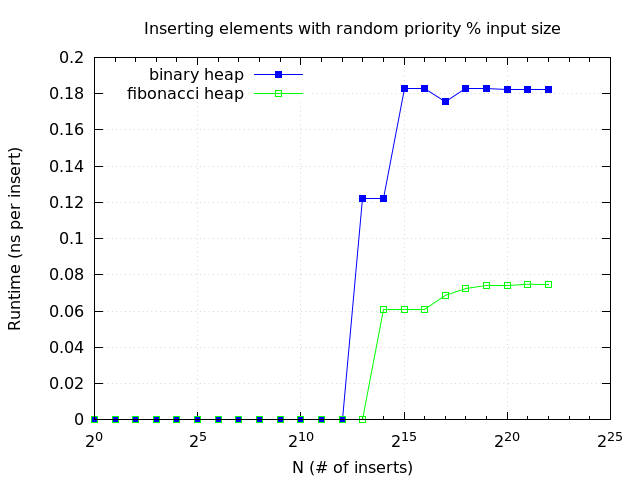
\includegraphics[width=\linewidth]{../res/inserts/insert_random_time_small.png}%
  \caption{INSERT TEXT}
  \label{fig:insert_t_random_small}
\end{minipage}%
\hfill
\begin{minipage}{0.48\columnwidth}
  \centering
  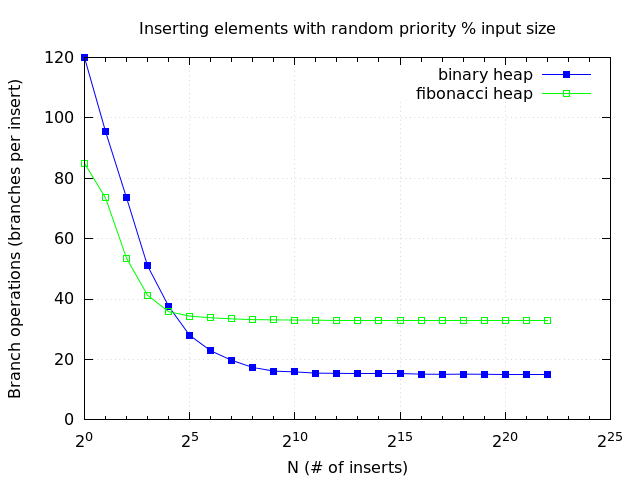
\includegraphics[width=\linewidth]{../res/inserts/insert_random_branch_small.png}%
  \caption{INSERT TEXT}
  \label{fig:insert_b_random_small}
\end{minipage}
\end{figure}

\begin{figure}[H]
\centering
  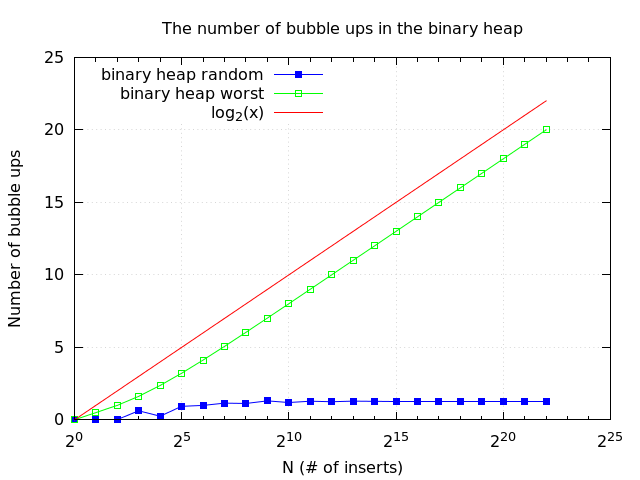
\includegraphics[scale=0.5]{../res/inserts/insert_bubble_up.png}%
  \caption{INSERT TEXT}
  \label{fig:bubble_ups}
\end{figure}

\subsection{\texttt{DeleteMin}}
Deleting the minimum element takes logarithmic time both priority queues. It can however take linear time in the worst case for the Fibonacci queue if a delete minimum operation is performed right after $n$ insert operations. We measure deleting the minimum in the average case where we randomly insert $n$ elements and then first pop one element from both queues such that the Fibonacci queue has consolidated. We then measure deleting one element for different heap sizes. We expect to see both have a logarithmic running time and logarithmic number of comparisons.
Testing in the worst case we will do the same but not consolidate the Fibonacci heap first and the binary heap should be inserted in sorted order.

We will also make an experiment where we fill the heap with $n$ elements and then pop them all again. This experiment is repeated 100 times and averaged where as the other with a single and two pops will be repeated 1000 times and averaged.

\begin{figure}[H]
\centering
\begin{minipage}{0.48\columnwidth}
  \centering
  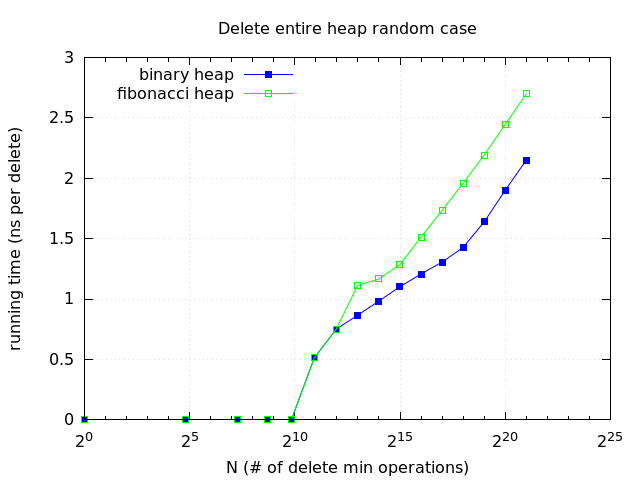
\includegraphics[width=\linewidth]{../res/delmin/delmin_del_all_time_random.png}%
  \caption{INSERT TEXT}
  \label{fig:delmin_all_random_time}
\end{minipage}%
\hfill
\begin{minipage}{0.48\columnwidth}
  \centering
  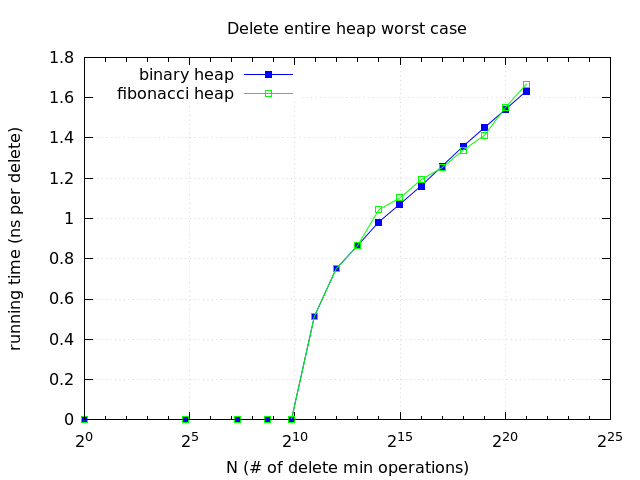
\includegraphics[width=\linewidth]{../res/delmin/delmin_del_all_time_worst.png}%
  \caption{INSERT TEXT}
  \label{fig:delmin_all_worst_time}
\end{minipage}
\end{figure}

\begin{figure}[H]
\centering
\begin{minipage}{0.48\columnwidth}
  \centering
  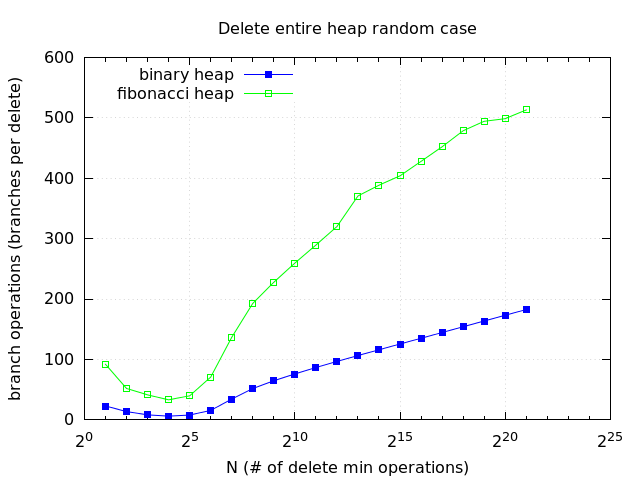
\includegraphics[width=\linewidth]{../res/delmin/delmin_del_all_branch_random.png}%
  \caption{INSERT TEXT}
  \label{fig:delmin_all_random_branch}
\end{minipage}%
\hfill
\begin{minipage}{0.48\columnwidth}
  \centering
  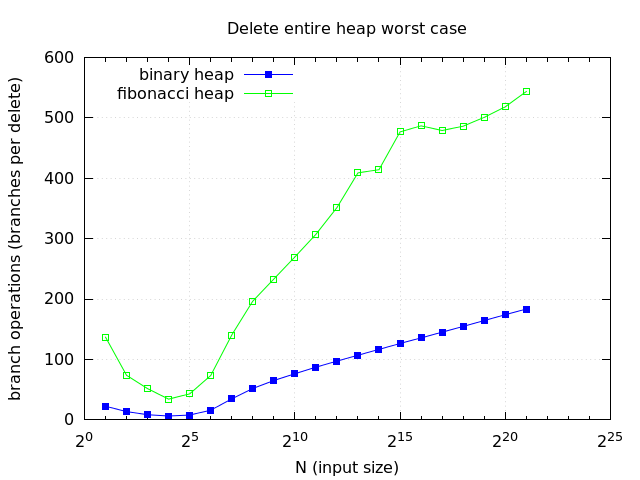
\includegraphics[width=\linewidth]{../res/delmin/delmin_del_all_branch_worst.png}%
  \caption{INSERT TEXT}
  \label{fig:delmin_all_worst_branch}
\end{minipage}
\end{figure}

\begin{figure}[H]
\centering
\begin{minipage}{0.48\columnwidth}
  \centering
  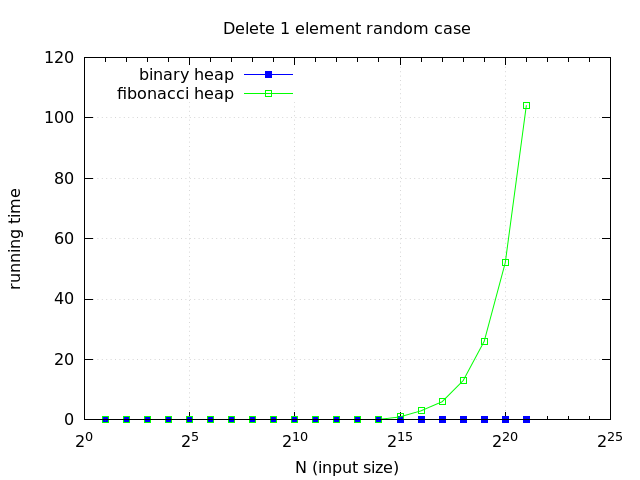
\includegraphics[width=\linewidth]{../res/delmin/delmin_del_1_time_random.png}%
  \caption{INSERT TEXT}
  \label{fig:delmin_1_random_time}
\end{minipage}%
\hfill
\begin{minipage}{0.48\columnwidth}
  \centering
  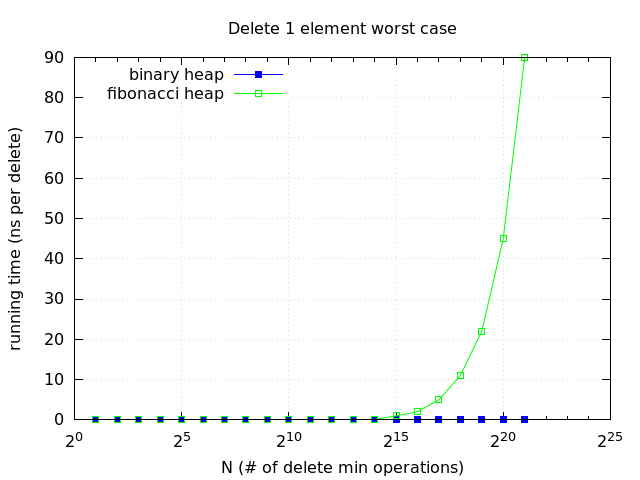
\includegraphics[width=\linewidth]{../res/delmin/delmin_del_1_time_worst.png}%
  \caption{INSERT TEXT}
  \label{fig:delmin_1_worst_time}
\end{minipage}
\end{figure}

\begin{figure}[H]
\centering
\begin{minipage}{0.48\columnwidth}
  \centering
  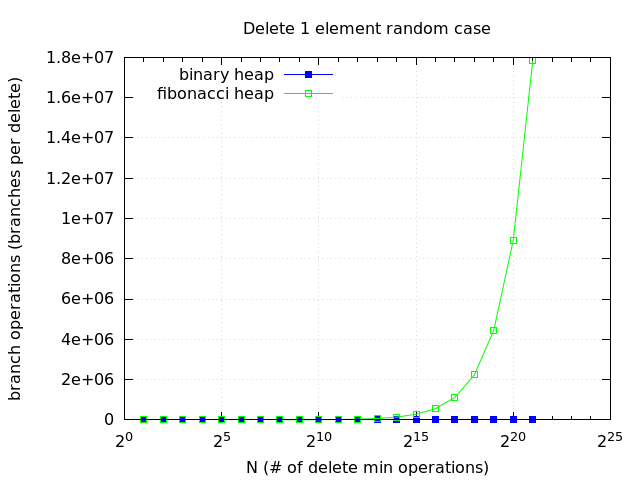
\includegraphics[width=\linewidth]{../res/delmin/delmin_del_1_branch_random.png}%
  \caption{INSERT TEXT}
  \label{fig:delmin_1_random_branch}
\end{minipage}%
\hfill
\begin{minipage}{0.48\columnwidth}
  \centering
  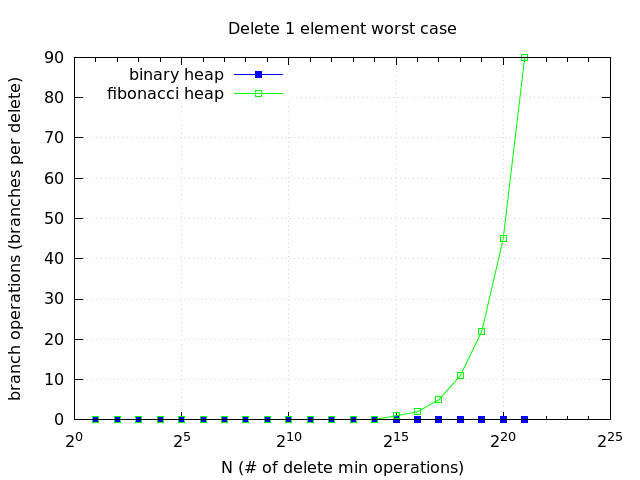
\includegraphics[width=\linewidth]{../res/delmin/delmin_del_1_branch_worst.png}%
  \caption{INSERT TEXT}
  \label{fig:delmin_1_worst_branch}
\end{minipage}
\end{figure}

\begin{figure}[H]
\centering
\begin{minipage}{0.48\columnwidth}
  \centering
  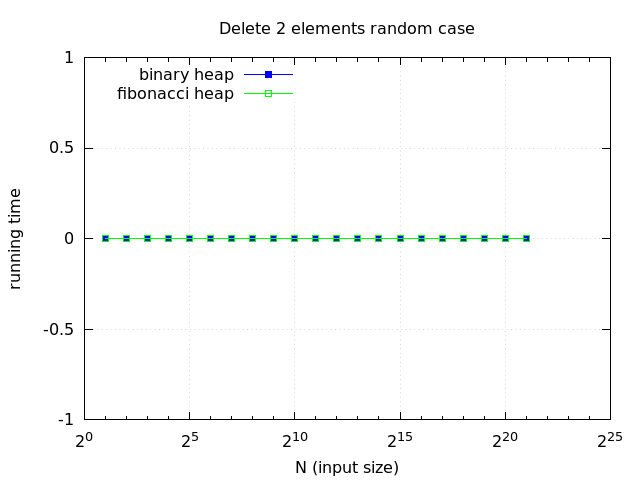
\includegraphics[width=\linewidth]{../res/delmin/delmin_del_2_time_random.png}%
  \caption{INSERT TEXT}
  \label{fig:delmin_2_random_time}
\end{minipage}%
\hfill
\begin{minipage}{0.48\columnwidth}
  \centering
  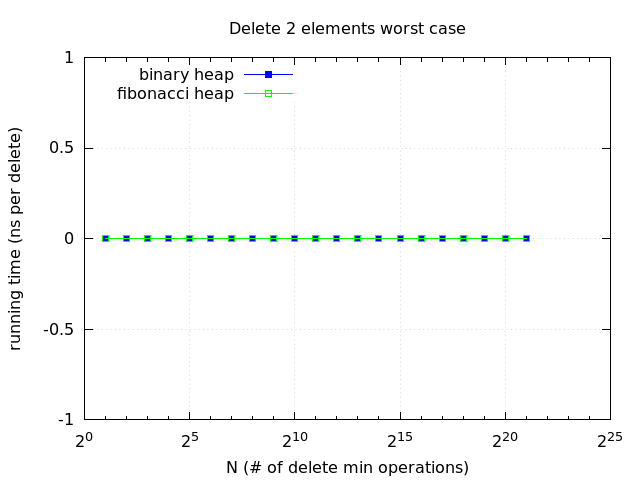
\includegraphics[width=\linewidth]{../res/delmin/delmin_del_2_time_worst.png}%
  \caption{INSERT TEXT}
  \label{fig:delmin_2_worst_time}
\end{minipage}
\end{figure}

\begin{figure}[H]
\centering
\begin{minipage}{0.48\columnwidth}
  \centering
  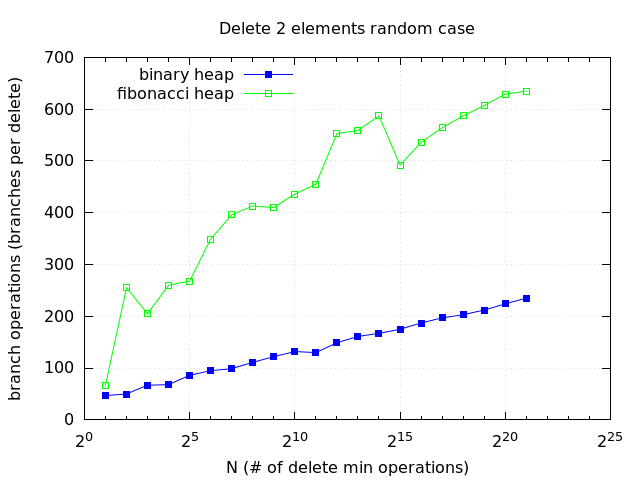
\includegraphics[width=\linewidth]{../res/delmin/delmin_del_2_branch_random.png}%
  \caption{INSERT TEXT}
  \label{fig:delmin_2_random_branch}
\end{minipage}%
\hfill
\begin{minipage}{0.48\columnwidth}
  \centering
  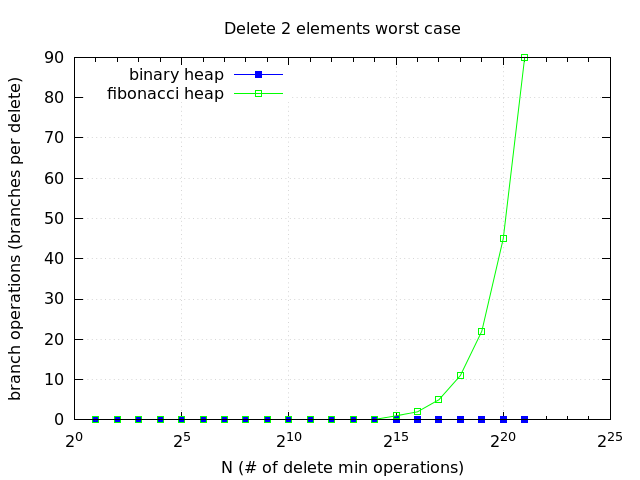
\includegraphics[width=\linewidth]{../res/delmin/delmin_del_2_branch_worst.png}%
  \caption{INSERT TEXT}
  \label{fig:delmin_2_worst_branch}
\end{minipage}
\end{figure}

Figure~\ref{fig:delmin_all_random_time} and ~\ref{fig:delmin_all_worst_time} shows that delete min takes logarithmic time in the size of the  input. The Fibonacci heap does however use a good deal more comparisons in both the random and the worst case as figure~\ref{fig:delmin_all_random_branch} and ~\ref{fig:delmin_all_worst_branch} shows.

Deleting one element from the Fibonacci heap after $n$ inserts is really expensive as figure~\ref{fig:delmin_1_random_time} and ~\ref{fig:delmin_1_random_branch} shows. This is also what we expected due to the really expensive consolidate that has to be run which takes linear time. We have the same picture in the worst case in figure~\ref{fig:delmin_1_worst_time} and ~\ref{fig:delmin_1_worst_branch}.

However if we first consolidate the Fibonacci heap by first performing a delete minimum which we do not measure and then run a delete min after we get the same running time as the binary heap. The results of this are shown in figure~\ref{fig:delmin_2_random_time},~\ref{fig:delmin_2_worst_time},~\ref{fig:delmin_2_random_branch}, and~\ref{fig:delmin_2_worst_branch}. It can be seen from the number of comparisons that the operations runs in logarithmic number of operations which is what we expected.

\subsection{\texttt{DecreaseKey}}
Decreasing the key in the Fibonacci heap should be amortized constant time as opposed to the logarithmic time in the binary heap. We would like to see this so we conduct an experiment where first randomly insert elements into the heap, and then perform some decrease key operations decreasing the key with some random number for a random element.

After that we will perform a worst case experiment. Here we will always decrease the key such that it will bubble to the top in the case of the binary heap. The worst case for the Fibonacci heap is really tricky to make a test case for, why the test will be the same as for the binary heap in the worst case.

\begin{figure}[H]
\centering
\begin{minipage}{0.48\columnwidth}
  \centering
  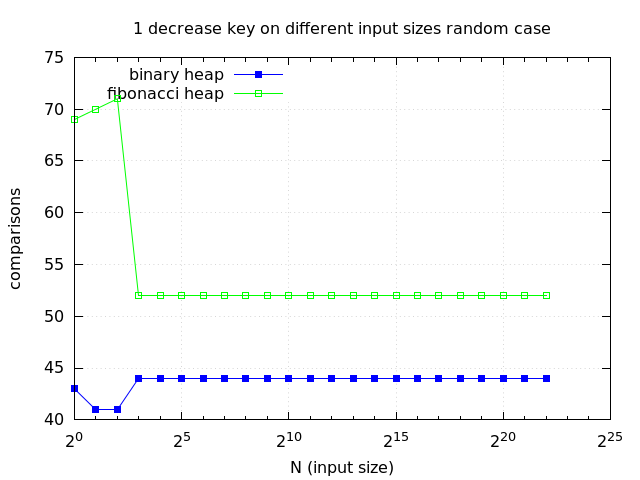
\includegraphics[width=\linewidth]{../res/dk/dk_random_fixed_size_1.png}%
  \caption{INSERT TEXT}
  \label{fig:dk_del_1_random}
\end{minipage}%
\hfill
\begin{minipage}{0.48\columnwidth}
  \centering
  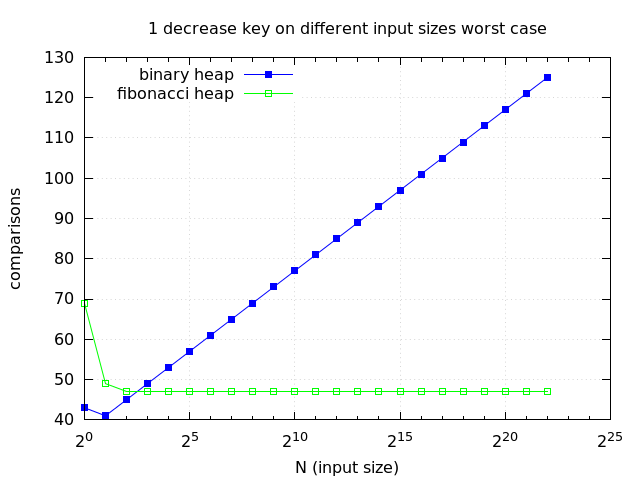
\includegraphics[width=\linewidth]{../res/dk/dk_worst_fixed_size_1.png}%
  \caption{INSERT TEXT}
  \label{fig:dk_del_1_worst}
\end{minipage}
\end{figure}

%TODO compiling using O2 makes bh better than fh but not in worst case MSP

\chapter{Dijkstra's algorithm}
In this section we introduce families of graphs that we believe makes Dijkstra's algorithm perform many respectively few \texttt{DecreaseKey} operations. It is obvious that the number of \texttt{DecreaseKey} operations is an exact measure of the number of edges we have to \textit{relax}.

\section{Few \texttt{DecreaseKey} operations}
\label{sec:few_decreasekey}
Since Dijkstra's algorithm finds shortest paths from the source $s$ to all vertices in the graph, we have to relax at least one ingoing edge for all other vertices. We therefore conclude that the lower bound for relaxing edges must be $\vert V \vert -1$. If not, the graph would contain unvisited vertices. Having a chain of vertices with \textit{weight} 0 on all edges causes Dijkstra to \textit{relax} each edge exactly once, giving us a graph with the desired property. It is clear that no additional (positive weighted) edges will be relaxed. For a graphical representation of the described class of graphs, please to figure~\ref{figure:graph_chain}. For future reference we denote this family of graphs \texttt{ChainGraphs}.

\begin{figure}[H]
\centering
\centerline {
  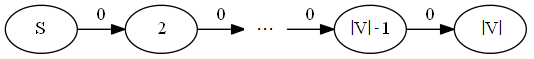
\includegraphics[scale=1]{../figures/graph_chain.png}
}
\caption{Chain of $\vert V \vert$ nodes with edge weight 0.}
\label{figure:graph_chain}
\end{figure}

\section{Many \texttt{DecreaseKey} operations}
\label{sec:many_decreasekey}
We consider an analysis of Dijkstra's algorithm using the fact that our implementation makes use of a priority queue $Q$. Since each vertex is removed from $Q$ exactly once, and the adjacency list of each vertex is scanned exactly once, it is clear that we can at most relax all edges exactly once.
In other words we need to consider graphs that makes Dijkstra's algorithm perform $\vert E \vert$ \texttt{DecreaseKey} operations in order to reach the upper bound.

We present two candidates of classes of graphs with the above mentioned property. The first proposal makes use of negative weights. Dijkstra's algorithm would still be able to run since we are not introducing negative cycles, but as we allow for previously marked nodes to be reinserted into the priority queue, we cannot rely on the asymptotic time bound. The second proposal uses only positive edge weights, and can therefore be compared against the asymptotic analysis.

\subsection{Candidate 1}
In the first candidate we split $n$ vertices into two sets $S_1, S_2$ of sizes $\lceil \nicefrac{(n-1)}{2} \rceil$ and $\lfloor \nicefrac{(n-1)}{2} \rfloor$ respectively. We now construct a chain of vertices from $S_1$. For chained vertex $v_i$ we have outgoing edge weight equal to $i$ for all $i \in [1, .. ,\lvert S_1 \lvert - 1]$. The last vertex on the chain has no outgoing edges for now. We now connect each vertex $v_i$ on the chain to all vertices ${v'}_i$ in $S_2$ with edge weight equal to $-2 \cdot i$. Finally we connect the source $s$ to $v_1$ in the chain with edge weight $n$ and to all ${v'}_i \in S_2$ with edge weight $n-1$. Please refer to figure~\ref{figure:graph_neg_weights} for an example with $n=6$. It is clear the example will make Dijkstra's algorithm relax all edges, and that this fact generalizes to graphs of arbitrary sizes.

\begin{figure}[H]
\centering
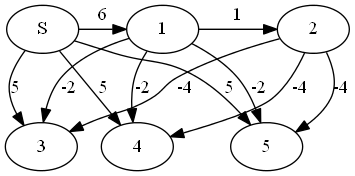
\includegraphics[scale=0.8]{../figures/graph_neg_weights.png}
\caption{Dijkstra's algorithm will have to relax all edges but we make us of negative edges}
\label{figure:graph_neg_weights}
\end{figure}

\subsection{Candidate 2}
In the second candidate we split $n$ vertices into three set $S_2, S_2$ and $S_3$ of sizes $\lceil \nicefrac{(n-1)}{3} \rceil$, $\lfloor \nicefrac{(n-1)}{3} \rfloor$ and $(n-1) - \lvert S_1 \rvert - \lvert S_2 \rvert$ respectively. We now construct a chain of vertices from $S_1$ with edge weight $0$. Connect each vertex $v_i$ on the chain to all vertices ${v''}_i \in S_3$ with edge weight equal to $n-2i$. Now connect each vertex ${v'}_i \in S_2$ to all vertices ${v''}_i \in S_3$ with edge weight $n^2 + 2n - 2i$ (we could have used $n^3$ for smaller $n$, but in order to avoid overflow we use this edge weight). Finally connect the source $s$ to the first vertex on the chain in $S_1$ with edge weight $n^2$ and to all vertices ${v'}_i \in S_2$ with edge weight $n+i$. Please refer to figure~\ref{figure:graph_pos_weights} for an example with $n=9$.  It is clear the example will make Dijkstra's algorithm relax all edges, and that this fact generalizes to graphs of arbitrary sizes. For future reference we denote this family of graphs \texttt{HeavyGraphs}

\begin{figure}[H]
\centering
\centerline {
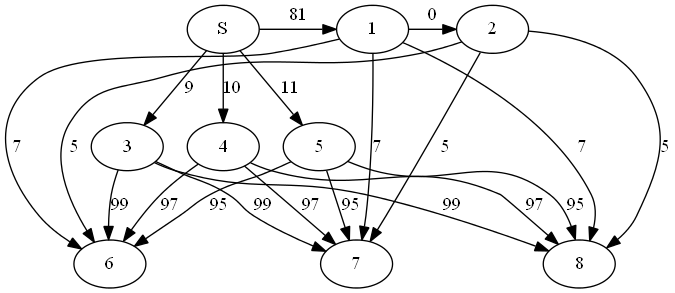
\includegraphics[scale=0.65]{../figures/graph_positive_weights.png}
}
\caption{Dijkstra's algorithm will have to relax all edges and we use only positive edges}
\label{figure:graph_pos_weights}
\end{figure}

\chapter{Experiments on Dijkstra's}
In this section we document the experiments done on Dijkstra's algorithm using both heap implementations. In particular we focus our studies on observing if the version using Fibonacci heaps achieves an improved performance because of the amortized $\mathcal{O}(1)$ time \texttt{DecreaseKey} operation. In the following we set $n = \lvert V \lvert$.

\section{Methodology}
We perform experiments using three families of graphs, namely \texttt{ChainGraphs} introduced in section~\ref{sec:few_decreasekey}, \texttt{HeavyGraphs} introduced in section~\ref{sec:few_decreasekey} and \texttt{RandomGraphs}. We will introduce the latter family in a short moment. Since we aim at comparing Dijkstra's algorithm on the different families, we started out by adding edges to the graphs such that they have equal number of edges on equal number of vertices. It is intuitively obvious that \texttt{HeavyGraphs} have more edges than \texttt{ChainGraphs}. A careful analysis tells us that graphs in \texttt{HeavyGraphs} with $\lvert V \rvert = n$ will have exactly $2(\nicefrac{n}{3})^2 + (\nicefrac{n}{3})-1$ edges. This gives reason for the following extensions of the constructions of each family.

\subsection{\texttt{ChainGraphs}}
We construct each graph as described in section~\ref{sec:few_decreasekey}. Furthermore we add $2(\nicefrac{n}{3})^2 + (\nicefrac{n}{3})- n - 2$ edges uniformly distributed over all vertices with edge weight $0$. This will make the graph have the desired total number of edges equal to graphs in \texttt{HeavyGraphs}. The extension will not make the graphs loose the property of making Dijkstra's algorithm perform few \texttt{DecreaseKey} operations.

\subsection{\texttt{HeavyGraphs}}
We construct each graph following the algorithm presented as \textit{Candidate 2} in section~\ref{sec:many_decreasekey}. Now further extensions is needed.

\subsection{\texttt{RandomGraphs}}
We construct each graph with $n$ vertices having $\dfrac{2(\nicefrac{n}{3})^2 + (\nicefrac{n}{3})-1}{n}$ outgoing edges. Each edge is connected uniformly random to another vertex. We avoid having edges connecting a vertex to itself and we avoid to have multiple outgoing edges to the same vertex. Edge weights are taken uniformly random in the interval $[0, .., 100]$. After construction we make sure that all components are connected. We do this by colouring all components and afterwards connecting different coloured components with a random edge. This scheme have a very limited overhead in number of extra edges.

\subsection{Experimental setup}
Please refer to chapter~\ref{chtp:experiment_setup} for a general overview of the experimental setup. We performed experiments on Dijkstra's algorithm using both heap implementations and using graphs from \texttt{ChainGraph}, \texttt{RandomGraph} and \texttt{HeavyGraph}. Each experiment was performed 5 times and the average was used.

\section{Expectations}
In general we expect Dijkstra's algorithm to achieve better running times, when using the Fibonacci heap, because of the amortised $\mathcal{O}(1)$ \texttt{DecreaseKey} operation. We expect to see the best running times on graphs from \texttt{ChainGraph} and the worst running times on graphs from \texttt{HeavyGraph} as argued in section~\ref{sec:few_decreasekey} and section~\ref{sec:many_decreasekey}. When running on graphs in \texttt{RandomGraph} we expect to see a slightly worse running time compared with runs on graphs from \texttt{ChainGraph}, but we expect to be far better than the runs on the worst case graphs from \texttt{HeavyGraph}.

\section{Results}

In figure~\ref{fig:dijkstra_chain_rt}, \ref{fig:dijkstra_random_rt} and \ref{fig:dijkstra_heavy_rt} we present plots of the total running time with Dijkstra on graphs with $\lvert V \lvert = N \in [2^2, 2^3, .., 2^{16}]$ on \texttt{ChainGraph}, \texttt{RandomGraph} and \texttt{HeavyGraph} respectively. In figure~\ref{fig:dijkstra_chain_rt_div_n}, \ref{fig:dijkstra_random_rt_div_n} and \ref{fig:dijkstra_heavy_rt_div_n} we present plots of the total running time divided by N. In figure~\ref{fig:dijkstra_chain_dk}, \ref{fig:dijkstra_random_dk} and \ref{fig:dijkstra_heavy_dk} we present plots of the total number of \texttt{DecreaseKey} operations initiated by Dijkstra's algorithm. In figure~\ref{fig:dijkstra_chain_br}, \ref{fig:dijkstra_random_br} and \ref{fig:dijkstra_heavy_br} we present the total number of conditional branches caused when running on \texttt{ChainGraph}, \texttt{RandomGraph} and \texttt{HeavyGraph} respectively. 

\begin{figure}[H]
\centering
\begin{minipage}{0.48\columnwidth}
  \centering
  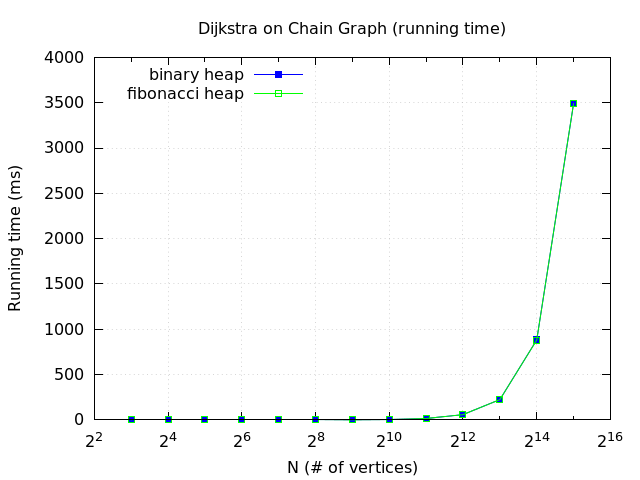
\includegraphics[width=\linewidth]{../res/dijkstra/d_chain_rt.png}%
  \caption{Dijkstra running time on ChainGraph}
  \label{fig:dijkstra_chain_rt}
\end{minipage}%
\hfill
\begin{minipage}{0.48\columnwidth}
  \centering
  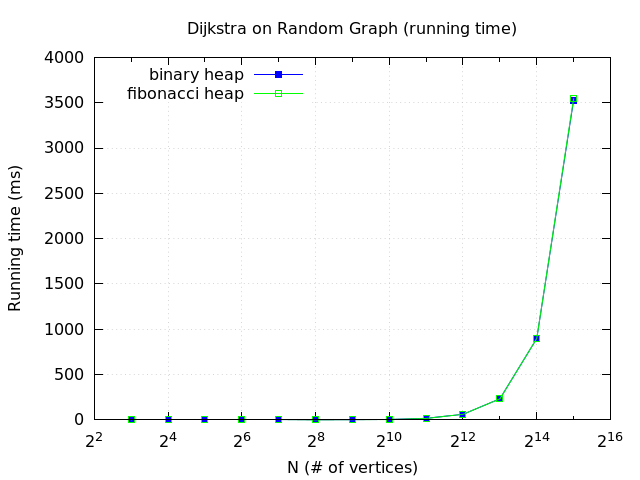
\includegraphics[width=\linewidth]{../res/dijkstra/d_random_rt.png}%
  \caption{Dijkstra running time on RandomGraph}
  \label{fig:dijkstra_random_rt}
\end{minipage}
\end{figure}

\begin{figure}[H]
\centering
\begin{minipage}{0.48\columnwidth}
  \centering
  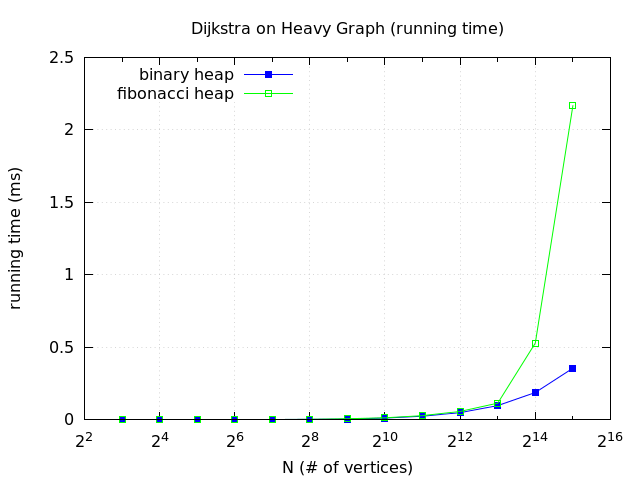
\includegraphics[width=\linewidth]{../res/dijkstra/d_heavy_rt.png}%
  \caption{Dijkstra running time on HeavyGraph}
  \label{fig:dijkstra_heavy_rt}
\end{minipage}%
\hfill
\begin{minipage}{0.48\columnwidth}
  \centering
  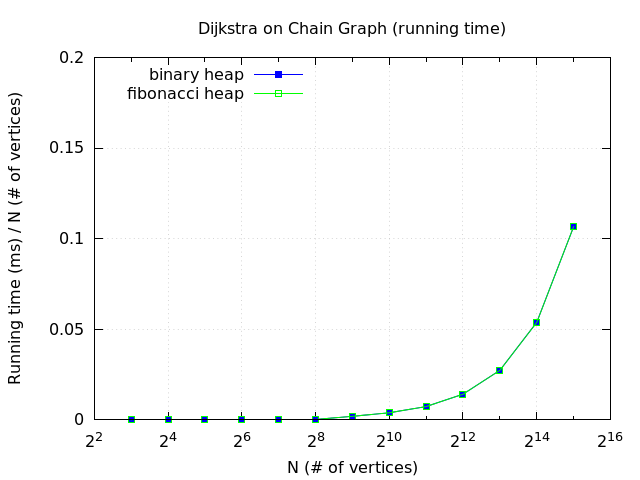
\includegraphics[width=\linewidth]{../res/dijkstra/d_chain_rt_div_n.png}%
  \caption{Dijkstra running time per vertex on ChainGraph}
  \label{fig:dijkstra_chain_rt_div_n}
\end{minipage}
\end{figure}

\begin{figure}[H]
\centering
\begin{minipage}{0.48\columnwidth}
  \centering
  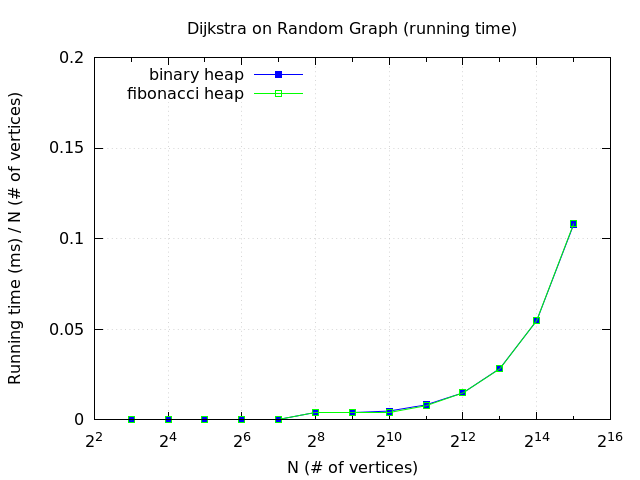
\includegraphics[width=\linewidth]{../res/dijkstra/d_random_rt_div_n.png}%
  \caption{Dijkstra running time per vertex on RandomGraph}
  \label{fig:dijkstra_random_rt_div_n}
\end{minipage}%
\hfill
\begin{minipage}{0.48\columnwidth}
  \centering
  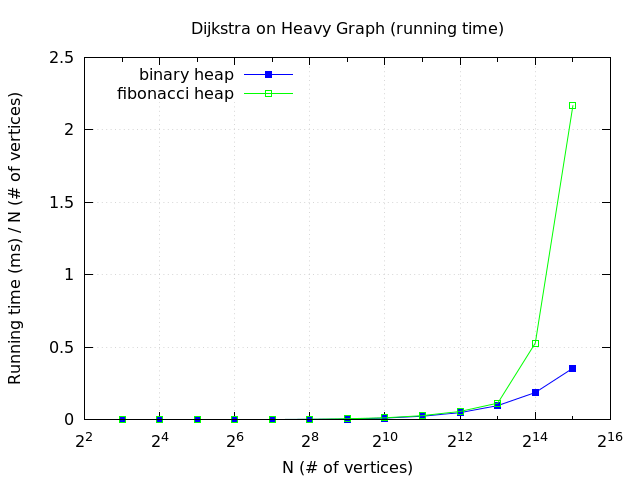
\includegraphics[width=\linewidth]{../res/dijkstra/d_heavy_rt_div_n.png}%
  \caption{Dijkstra running time per vertex on HeavyGraph}
  \label{fig:dijkstra_heavy_rt_div_n}
\end{minipage}
\end{figure}

\begin{figure}[H]
\centering
\begin{minipage}{0.48\columnwidth}
  \centering
  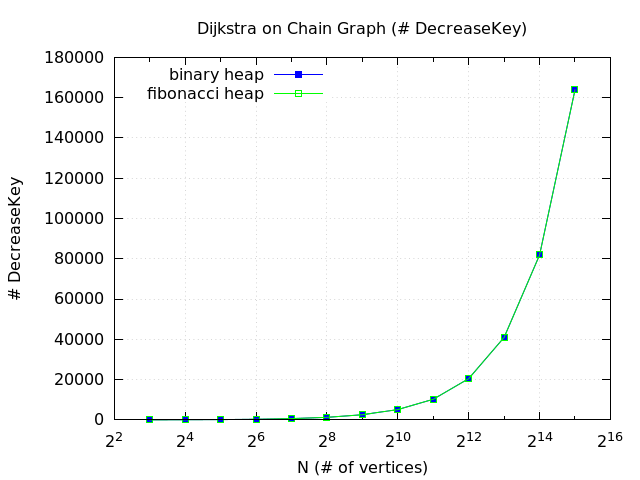
\includegraphics[width=\linewidth]{../res/dijkstra/d_chain_dk.png}%
  \caption{DecreaseKey operations on ChainGraph}
  \label{fig:dijkstra_chain_dk}
\end{minipage}%
\hfill
\begin{minipage}{0.48\columnwidth}
  \centering
  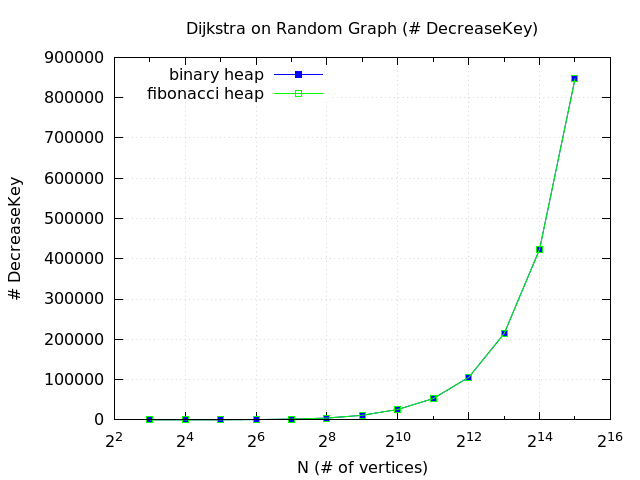
\includegraphics[width=\linewidth]{../res/dijkstra/d_random_dk.png}%
  \caption{DecreaseKey operations on RandomGraph}
  \label{fig:dijkstra_random_dk}
\end{minipage}
\end{figure}

\begin{figure}[H]
\centering
\begin{minipage}{0.48\columnwidth}
  \centering
  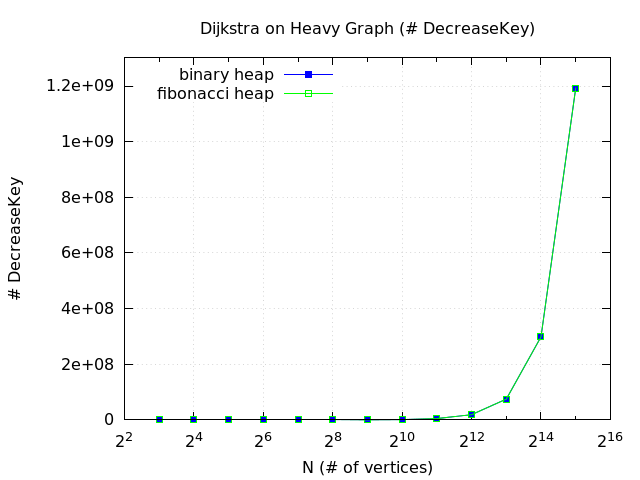
\includegraphics[width=\linewidth]{../res/dijkstra/d_heavy_dk.png}%
  \caption{DecreaseKey operations on HeavyGraph}
  \label{fig:dijkstra_heavy_dk}
\end{minipage}%
\hfill
\begin{minipage}{0.48\columnwidth}
  \centering
  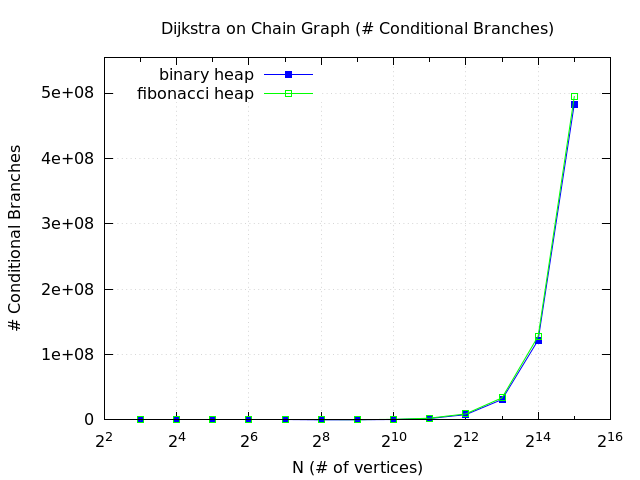
\includegraphics[width=\linewidth]{../res/dijkstra/d_chain_br.png}%
  \caption{Conditional Branches on ChainGraph}
  \label{fig:dijkstra_chain_br}
\end{minipage}
\end{figure}

\begin{figure}[H]
\centering
\begin{minipage}{0.48\columnwidth}
  \centering
  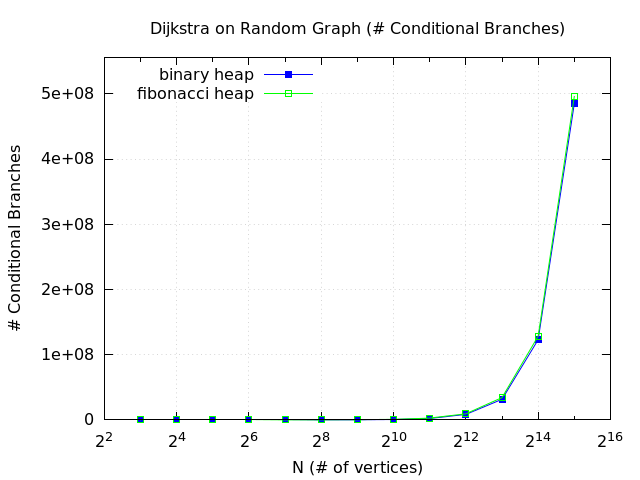
\includegraphics[width=\linewidth]{../res/dijkstra/d_random_br.png}%
  \caption{Conditional Branches on RandomGraph}
  \label{fig:dijkstra_random_br}
\end{minipage}%
\hfill
\begin{minipage}{0.48\columnwidth}
  \centering
  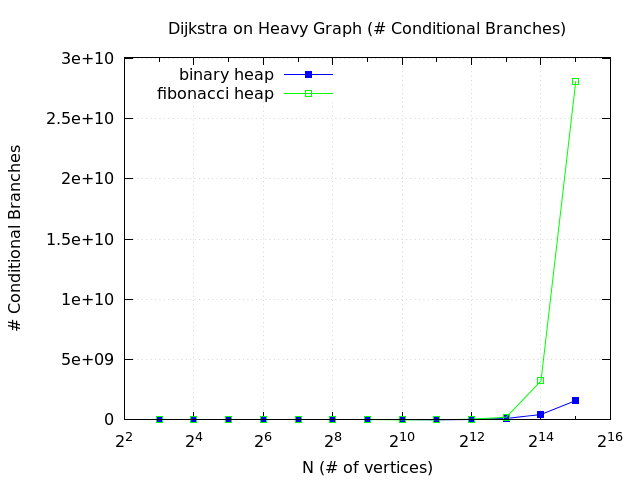
\includegraphics[width=\linewidth]{../res/dijkstra/d_heavy_br.png}%
  \caption{Conditional Branches on HeavyGraph}
  \label{fig:dijkstra_heavy_br}
\end{minipage}
\end{figure}

\section{Discussion}
Comparing the running times on \texttt{ChainGraph} respectively \texttt{RandomGraph} in figure~\ref{fig:dijkstra_chain_rt} and \ref{fig:dijkstra_random_rt} we see that our hypothesis of seeing close to the same running times on graphs from \texttt{ChainGraph} and \texttt{RandomGraph} holds. We are surprised to see that the running times is almost the exact same for both heap implementations. We believe we see this behaviour because we have chosen graphs with relatively few vertices. Furthermore we have implemented Dijkstra's algorithm such that it fills 

\bibliography{references}

\end{document}


